% !TEX program = xelatex
% AAAI 2026 双栏中文排版预览。
% 本文件因中文内容使用 XeLaTeX，仅供工作稿审阅；正式投稿应使用独立英文 PDFLaTeX 稿。
\documentclass[letterpaper]{article}
% 复用项目内未修改的 AAAI 2026 官方样式文件。
\usepackage[submission]{aaai2026_prism/aaai2026}
\usepackage{times}
\usepackage{helvet}
\usepackage{courier}
\usepackage[hyphens]{url}
\urlstyle{rm}
\def\UrlFont{\rm}

% XeLaTeX 中文支持；不用 ctex/geometry/hyperref，以保持 AAAI 样式的版芯和限制。
\usepackage{xeCJK}
\setCJKmainfont[
  BoldFont=SimHei,
  ItalicFont=KaiTi,
  BoldItalicFont=KaiTi
]{SimSun}
\setCJKsansfont[BoldFont=SimHei]{SimHei}
\setCJKmonofont{SimSun}

\usepackage{amsmath,amssymb,amsthm}
\usepackage{booktabs}
\usepackage{multirow}
\usepackage{graphicx}
\usepackage{tikz}
\usetikzlibrary{arrows.meta, positioning, shapes.geometric}
\frenchspacing
\setlength{\pdfpagewidth}{8.5in}
\setlength{\pdfpageheight}{11in}
\pdfinfo{
/TemplateVersion (2026.1)
}

% ---------- 常用宏 ----------
\newcommand{\method}{SPARC}
\newcommand{\sbw}{SBW}
\newcommand{\zthree}{Z3}
\newcommand{\Sol}{\mathrm{Sol}}
\newcommand{\AnsSol}{\mathrm{Sol}_{A}}
% 占位宏（正文用例已全部清空并转为正规叙述）：保留为安全网，残留时以正常文本排版。
\newcommand{\TODO}[1]{#1}
% 默认只编译 AAAI 主文证据；设为 \includeexploratorytrue 可显示历史审计账本。
\newif\ifincludeexploratory
\includeexploratorytrue % 工作稿显示探索性附录；投稿前改回 \includeexploratoryfalse

\newtheorem{definition}{定义}
\newtheorem{proposition}{命题}
\renewcommand{\refname}{参考文献}

% ==== AAAI 英文标题：当前生效为最后一行的 \title；其余为备选 ====
\title{Satisfiable but Wrong: Solver-Decidable Abstention for LLM Constraint Formalization}
\author{匿名作者}

\begin{document}
\maketitle

\begin{abstract}
神经符号约束推理通常将 LLM 生成的约束交给求解器，并在返回 SAT 后接受答案；但
SAT 只保证生成约束彼此一致，不保证其忠实表达题意，遗漏或弱化线索仍会产生可满足、
但任务层面错误（satisfiable-but-wrong，\sbw{}）的答案，而以语法错误或 UNSAT 为触发
条件的修复无法识别这类仍保持 SAT 的信息遗漏。本文研究一个更窄的问题：在不读取实例
答案值的前提下，任务规范能否提供由求解器判定的 SAT 后拒答条件？为此我们提出
\method{}：对要求唯一答案的任务，它以一次增量阻塞子句查询判定答案投影是否唯一
（无需枚举全部解），将确定的非唯一状态映射为结构性拒答，并把确定通过、结构性拒答与
UNKNOWN 明确分开。在 ZebraLogic 冻结的无门控 SAT 状态上，唯一性探针在不依赖答案模式
预校验的保守口径下检出 baseline 与 aggressive 输出中 81.3\% 与 82.3\% 的已观测
\sbw{}（启用该预校验的筛后口径为 92.3\% 与 94.5\%），代价是将 9.7\% 与 23.8\% 的正确
输出转为结构性拒答；在一个 78 题金标子集的所报告操作点上，门控以单次形式化取得低于
口头置信度与多形式化一致性基线的作答风险，且无需额外 LLM 调用。结果将唯一答案任务的
答案投影唯一性定位为一种可判定的选择性作答信号，而非语义正确性、端到端修复收益或
跨任务泛化的证据。
\end{abstract}

\section{引言}
\label{sec:intro}

自然语言约束推理要求系统从题面恢复变量、关系和全局约束，再由形式求解器生成
答案。Logic-LM~\cite{pan2023}、LINC~\cite{olausson2023} 和 SatLM~\cite{ye2023}
分别将 LLM 与逻辑程序、一阶逻辑证明器和可满足性求解器结合，使生成的形式表示能够
由求解器复核。在基于可满足性求解的流水线中，系统通常将 SAT 作为接受答案的依据
~\cite{pan2023,ye2023}。

这一接受规则存在明确盲区：SAT 只说明生成约束彼此一致，不说明它们表达了题意。
当线索被遗漏或弱化时，系统仍可能输出可满足、但任务层面错误的作答，即可满足但错误
（satisfiable-but-wrong，\sbw{}）~\cite{wei2025}。以语法错误、执行失败或 UNSAT 等
显式反馈为触发条件的修复流程可以处理冲突，却无法仅凭这些反馈识别仍保持 SAT 的
信息遗漏~\cite{kirtania2024,singh2026}。

\begin{figure}[t]
  \centering
  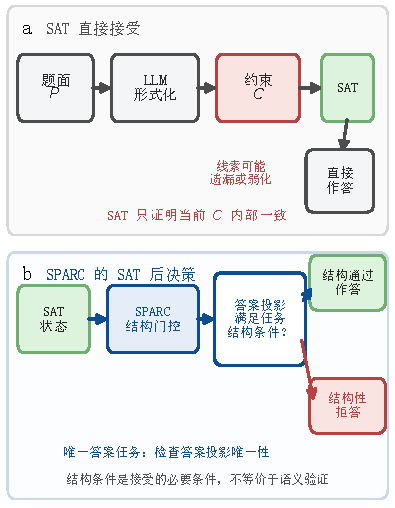
\includegraphics[width=\columnwidth]{figures/fig_motivation}
  \caption{\method{} 的动机与决策位置。(a) SAT 只验证当前生成约束的内部一致性；
  线索遗漏或弱化后，系统仍可能直接接受一个可满足的作答。(b) \method{} 在 SAT 后
  检查由任务规范给出的答案空间结构条件；在唯一答案任务中，非唯一答案投影触发结构性
  拒答。该门控不读取答案值，也不构成语义验证。}
  \label{fig:motivation}
\end{figure}

上述修复路线关注如何新增、修改或重写约束；语义对齐路线则直接评估题面文本与形式
表示是否一致，例如学习式评分、符号等价、往返一致性和多次形式化一致性
~\cite{lu2025,li2024symbolic,ryu2025,raza2025,zhou2024dtv}。另一类选择性作答方法
根据置信度估计~\cite{xiong2024,zhang2024rtuning}或多次采样一致性
~\cite{wang2023,manakul2023}决定何时保留输出。本文与这些路线互补：不尝试定位遗漏
线索或直接证明语义等价，而是在已有 SAT 状态上检查任务规范给出的结构条件。

本文因此研究一个更窄的问题：在不访问实例答案值的前提下，系统何时应拒绝一个 SAT
结果？该问题将“约束内部一致”与“任务答案正确”分开，并将目标转化为寻找可判定的拒答
依据，属于选择性预测（selective prediction）~\cite{chow1957,geifman2017,kamath2020}。
为此，本文提出 \method{}。如图~\ref{fig:motivation} 所示，在唯一答案任务中，系统在
答案变量集合上构造阻塞子句以查询是否存在第二个答案投影；确定唯一时接受，确定非唯一
时结构性拒答，并将 UNKNOWN 单独记录。该门控只改变 SAT 后的接受条件，不替换基础
形式化器或求解器。我们在冻结约束状态上测量其检出范围和覆盖率代价，并在共享问题集上
与启发式拒答信号比较。

本文的主要贡献如下：
\begin{itemize}
  \item \textbf{界定 \sbw{} 的可诊断边界。}在唯一答案、纯欠约束的前提下，答案投影
        必然非唯一；唯一但错的 SAT 输出会逃逸唯一性门控。
  \item \textbf{提出 \method{} 的 SAT 后结构门控。}以答案投影唯一性构造无需训练、
        不读取金标答案值且由求解器可判定的拒答接口。
  \item \textbf{量化结构门控的检出范围和代价。}在冻结的 ZebraLogic SAT 状态上报告
        \sbw{} 检出与正确输出拒答，并在风险--覆盖率下与启发式拒答基线比较。
\end{itemize}

% ============================================================
% 相关工作按机制而非文献清单组织。
% ============================================================
\section{相关工作}
\label{sec:related}

\subsection{LLM 约束形式化}
把自然语言映射为形式表示的自动形式化~\cite{wu2022} 催生了一条神经符号路线：让 LLM
只负责翻译、由求解器负责推理，从而规避直接长链推理累积的中间不一致~\cite{lin2025,tyagi2024}。
代表性系统按目标形式分化——Logic-LM~\cite{pan2023} 生成逻辑程序，LINC~\cite{olausson2023}
生成一阶逻辑并交给证明器，SatLM~\cite{ye2023} 生成可满足性约束；后续工作把这一范式推广
到领域专用语言~\cite{kesseli2025}、统一求解器接口~\cite{callewaert2025}、SMT~\cite{oh2026}，
以及约束建模~\cite{tsouros2023,michailidis2024} 与优化建模~\cite{ahmaditeshnizi2024}。这类
方法的共同优势是把推理外包给可靠求解器、使中间结果可复核；其共同盲区是，可复核的只是
求解器状态而非题意——SATBench 表明，即使线索被遗漏，欠约束的形式化仍会返回
SAT~\cite{wei2025}。因此本文不追求一般的语义忠实性，而是在这一 SAT 盲区中界定并处理
一个\emph{可判定}的子问题。

\subsection{形式化的验证与修复}
为纠正错误形式化，一条路线让模型自反馈复审自身输出~\cite{madaan2023,shinn2023}，但受控
研究显示自我纠错在推理与代码任务上并不稳定~\cite{huang2024,olausson2024}；另一条路线改用
求解器的显式失败信号——不可满足核或冲突子集——来定位并修复约束，既见于逻辑形式化的
迭代修复~\cite{kirtania2024,singh2026}，也见于优化模型的不可行诊断与修正
~\cite{chen2024optichat,zhang2025sacopt,ao2026}。这两支修复的共同局限在于\emph{触发条件}：
它们依赖语法错误、执行失败或 UNSAT，因而对仍保持 SAT 的信息遗漏无从察觉。与之互补，
语义对齐路线绕过求解器状态、直接比较题面与形式表示，如学习式对齐评分~\cite{lu2025}、
符号等价~\cite{li2024symbolic}、翻译回环一致性~\cite{ryu2025,zhou2024dtv} 与多次形式化
一致性~\cite{raza2025}；它们能覆盖更广的语义偏差，但代价是需要文本--形式比较、额外模型
或多次采样。本文与两者都不冲突：\method{} 既不定位缺失线索、也不判定语义等价，而是只
检查答案空间的结构条件——结论严格弱于语义验证，但只需一次求解器判定即可得出。

\subsection{选择性预测}
在不确定时选择拒答（选择性预测）由 Chow~\cite{chow1957} 提出，并在深度模型上以风险--
覆盖率框架形式化~\cite{geifman2017,kamath2020}。面向 LLM 的拒答信号大多是启发式的：或
读取自评置信度~\cite{xiong2024,zhang2024rtuning}，或统计多次采样的一致性
~\cite{wang2023,manakul2023}；其共同弱点是需要额外采样或诱导、且判定本身带有随机性
~\cite{wen2024}。与“从模型不确定性取信号”不同，另一支工作从\emph{解空间结构}取信号：
解枚举用于多解实例评分与歧义审计~\cite{amonkar2025,hall2026}，而最小不可满足子集
~\cite{liffiton2008}、约束获取~\cite{bessiere2013,tsouros2024} 与 oracle 引导的程序合成
（CEGIS）~\cite{jha2010} 则用可区分模型（两个满足当前约束却不同的解）主动补充约束——
但后者假设一个可信 oracle。\method{} 把这两支接起来：它用求解器对答案投影\emph{非唯一性}
的确定判定作为拒答信号，无需采样、可与上述启发式基线在同一风险--覆盖率坐标系下比较；
而它借用的可区分模型只驱动探索性候选补全，且因 LLM 并非可信 oracle，本文不将该补全
表述为修复器。

\section{\method{}：SAT 后结构门控}
\label{sec:method}
\label{sec:problem}

\subsection{问题设定与可诊断的错误}
\label{sec:setting}

给定自然语言问题 $P=(B,L)$，其中 $B$ 是背景描述，
$L=\{l_1,\ldots,l_m\}$ 是线索集合。LLM 形式化器 $T$ 生成约束集
$C=T(P)$，求解器返回满足 $C$ 的模型。模型可能包含辅助变量，因此本文在
答案变量集合 $V_A$ 上定义投影解空间：
\begin{equation}
  \AnsSol(C)=\{M|_{V_A}: M\models C\}.
\end{equation}
下文将 $S=\AnsSol(C)$ 记为当前编码的答案投影空间。
为讨论补全的搜索进展，记完整模型空间为
\begin{equation}
  \Sol(C)=\{M:M\models C\}.
\end{equation}
系统输出 $\hat A\in\AnsSol(C)$，或在没有可接受答案时返回非作答状态。
理论上，$V_A$ 应由任务接口显式给出。在 ZebraLogic 中，它对应实体到房间位置
的整数变量，求解器追踪变量不参与答案投影或唯一性阻塞子句。本文实验所用的
历史实现以全部非追踪整数变量近似这一集合（当前实现已支持从可见题面推导、
不读金标的答案变量白名单，见 \S\ref{sec:limitations}），故本文关于唯一性的
实证结论仅适用于该基准的当前编码；其他任务必须提供答案变量白名单。

记 $C^{*}$ 为忠实表达 $P$ 的约束集，$S^{*}=\AnsSol(C^{*})$ 为真实答案
空间。任务规范可提供结构先验 $\pi$，其对应答案空间谓词为 $g_{\pi}(S)$，
且不包含具体答案：ZebraLogic 使用 $g_{\pi}(S)=[|S|=1]$，选择题任务可用
候选数或题型判定模式定义 $g_{\pi}$。结构门控只检查该谓词 $g_{\pi}(S)$，
不比较 $S^{*}$ 中的答案值。

ZebraLogic 的具体答案模式校验、金标接口和由此带来的实验边界在
\S\ref{sec:setup} 中说明；它们不属于上述问题定义或结构谓词本身。

在此设定下，我们进一步区分可诊断与不可诊断的错误。
\label{sec:prior}

\begin{definition}[\sbw{} 失败]
\label{def:sbw}
若 $\AnsSol(C)\neq\emptyset$ 且系统输出 $\hat A\notin S^{*}$，则该次运行
发生 satisfiable-but-wrong（\sbw）失败。该定义刻画的是任务层面的输出
错误：求解器对 $C$ 的 SAT 判断仍然正确，错误发生在 $C$ 未忠实表达 $P$ 或
系统从该状态给出了错误答案。
\end{definition}

测试时无法比较 $S$ 与 $S^{*}$，但可以检查 $g_{\pi}(S)$。在唯一答案任务中，
纯欠约束与答案投影非唯一之间存在以下直接关系。

\begin{proposition}[纯欠约束的可检出性]
\label{prop:underconstraint}
若任务真实答案唯一，即 $|S^{*}|=1$，且当前编码只遗漏或弱化约束而未排除真实
答案，使得 $S^{*}\subsetneq S$，则 $|S|>1$。因此，唯一性门控将确定地拒答。
\end{proposition}
\begin{proof}
由 $S^{*}\subsetneq S$ 可知 $S$ 至少包含 $S^{*}$ 中的唯一答案以及一个不同的
额外答案投影，故 $|S|>1$。
\end{proof}

\begin{proposition}[唯一但错的逃逸边界]
\label{prop:unique-wrong}
若 $|S|=1$，但系统输出的唯一答案 $\hat A\notin S^{*}$，则唯一性门控通过，
却不能识别该 \sbw{}。
\end{proposition}
\begin{proof}
唯一性门控只计算 $|S|$，不比较 $\hat A$ 与 $S^{*}$。在 $|S|=1$ 时，门控的
接受条件成立，即使该唯一投影在任务层面错误。
\end{proof}

这些命题的逆命题均不成立：多个答案也可能来自混合误约束、变量建模错误或错误的
答案投影。因此，非唯一是结构异常证据，而不是对缺失线索的语义定位。

同样，$g_{\pi}(S)$ 成立只是接受答案的必要条件。答案投影唯一但仍错误的
SAT 输出会通过门控。方法依赖三个前提：任务先验有效、答案投影完整且求解器
能在预算内给出确定判定。违反任一前提都会削弱结论。候选补全或冲突处理若只
以恢复 SAT 为目标，也可能弱化题意约束；因此它们不能据此被称为语义修复。

\subsection{整体框架与系统流程}
\label{sec:method-setup}

\method{} 位于基础“形式化--求解--修复”流水线之后。它接收已判定 SAT 的约束集，
先在答案投影上检查任务结构条件，再决定接受、拒答或进入可选的探索性补全分支。
给定自然语言问题 $P$、约束集 $C$、答案变量集合 $V_A$ 与结构先验谓词 $g_{\pi}$，
系统将 SAT 后状态映射为以下三类输出：
\begin{itemize}
  \item \emph{结构通过的答案}：一个约束集 $C'$ 与答案 $\hat A\in\AnsSol(C')$，
        其中 $C'$ 为 SAT，且求解器已确定 $g_{\pi}(\AnsSol(C'))$ 成立；
  \item \emph{结构性拒答}：求解器确定 $g_{\pi}(\AnsSol(C'))$ 不成立；
  \item \emph{未验证兼容输出}：门控返回 UNKNOWN 或无法构造答案投影时，历史
        实现沿用基础流水线输出并记录状态。该分支不属于上述结构通过的答案，也不
        用于支持本文的结构门控结论。
\end{itemize}

结构条件是接受答案的必要条件而非充分条件：\method{} 不比较真实答案空间
$S^{*}$，因而只能拦截可判定的结构违规，不能证明 $C'$ 语义正确。该接口还
将确定的门控通过同 UNKNOWN 或投影构造失败显式分开；面向部署的系统可将后者
报告为未验证输出，或采用 fail-closed 策略。本文的冻结状态诊断只统计可得到
确定答案投影的 SAT 状态。

\label{sec:statemachine}

\begin{figure*}[t]
  \centering
  \resizebox{\textwidth}{!}{%
  \begin{tikzpicture}[
      font=\small,
      node distance=12mm and 10mm,
      box/.style={draw, rounded corners=2pt, align=center, inner sep=4pt},
      mod/.style={box, fill=gray!12},
      expl/.style={box, fill=gray!5, dashed},
      term/.style={box, fill=gray!25},
      arr/.style={-{Stealth}, semithick},
    ]
    \node[box] (t) {LLM 形式化\\$C=T(P)$};
    \node[box, right=of t] (solve) {求解与基础修复};
    \node[mod, right=of solve] (gate) {结构门控};
    \node[term, right=of gate, text width=21mm] (accept) {结构通过\\的答案};
    \node[expl, below=of solve] (core) {启发式\\冲突处理};
    \node[expl, below=of gate] (diff) {模型差分\\候选补全};
    \node[term, below=of accept] (abstain) {非作答};
    \draw[arr] (t) -- (solve);
    \draw[arr] (solve) -- node[above] {SAT} (gate);
    \draw[arr] (gate) -- node[above, font=\footnotesize, pos=.35] {$g_{\pi}$ 成立} (accept);
    \draw[arr] (gate.south west) to[bend right=18]
      node[left, font=\footnotesize, align=right] {第二答案\\模型} (diff.north west);
    \draw[arr] (gate.south east) to[bend left=16]
      node[right, font=\footnotesize, align=left] {确定非唯一\\（$K=0$）} (abstain.north);
    \draw[arr] (diff.north east) to[bend right=18]
      node[right, font=\footnotesize, align=left] {补全后\\SAT} (gate.south east);
    \draw[arr] (diff.west) -- node[above, font=\footnotesize] {UNSAT} (core.east);
    \draw[arr] (core.north) -- node[left, font=\footnotesize, align=right]
      {修复后\\重求解} (solve.south);
    \draw[arr] (diff) -- node[below, font=\footnotesize, align=center]
      {失败或\\预算耗尽} (abstain);
    \draw[arr, dashed, gray] (solve.north) to[bend left=18]
      node[above, font=\footnotesize, text=gray] {基础流水线：SAT 直接接受} (accept.north);
  \end{tikzpicture}}
  \caption{\method{} 的结构门控流程。灰色点划线表示基础流水线在 SAT 后直接
  接受答案。\method{} 先检查答案空间是否满足结构先验；确定唯一则接受，确定非
  唯一则结构性拒答。虚线灰框（冲突处理、候选补全）为探索性扩展，不参与本文的
  门控诊断结论。图中“结构通过的答案”仅表示求解器确定通过门控的情形；UNKNOWN
  和无法构造投影时的兼容输出未画出。}
  \label{fig:framework}
\end{figure*}

图~\ref{fig:framework} 展示了从 SAT 状态到输出决策的路径。门控先检查
$g_{\pi}$；在未启用候选补全时，确定非唯一直接导致结构性拒答；启用该探索性
分支时，系统先尝试候选补全，再对新的 SAT 状态重新门控。模型差异
只是候选约束的局部提示，而非缺失线索的确定定位。候选引发冲突时，处理例程
优先修改早期约束；任何重新得到的 SAT 状态都必须再次经过门控。与基础流水线
相比，\method{} 改变的是答案的接受条件，而非形式化器或底层求解器。

\subsection{核心机制：结构先验门控}
\label{sec:pigate}

门控的设计依据来自 \S\ref{sec:prior}：SAT 只保证约束集内部一致，而
$g_{\pi}$ 是不依赖实例答案、可由求解器判定的必要条件。对唯一答案
任务，判定答案投影是否唯一不需要枚举全部解，只需一次带阻塞子句的
增量求解。具体地，门控先取得模型 $M$，再构造答案阻塞子句
\begin{equation}
  \beta(M)=\lnot\bigwedge_{v\in V_A}(v=M[v]).
\end{equation}
若 $C\cup\{\beta(M)\}$ 为 UNSAT，则 $M|_{V_A}$ 是唯一答案投影，结构检查
确定通过。若结果为 SAT，求解器返回第二个答案模型 $M'$。当 $K=0$ 时，系统直接
结构性拒答；仅在启用探索性候选补全且预算尚未耗尽时，$M'$ 才作为该分支的输入。
阻塞只覆盖 $V_A$；若将辅助变量加入阻塞子句，同一任务答案的不同内部赋值
会被误判为多个答案。

本文报告的实验将全部非追踪整数决策变量视为 $V_A$，这一近似与当前实现新增的
白名单口径见 \S\ref{sec:limitations}。求解超时时，实现采用放行并记录 UNKNOWN 的策略。
这保留了基础流水线的覆盖率，但该输出不具备唯一性保证，也不计为结构门控通过。

在选择题中，$g_{\pi}$ 可由选项谓词的判定模式实现。以 could-be-true 为例，
系统分别检查每个选项与背景约束的可满足性，并要求候选集合符合题目规定的
良定模式。该实例化不使用唯一性阻塞子句，但仍遵循先检查结构条件、再决定
是否输出的流程；UNKNOWN 仍需与确定通过的结果区分记录。

\subsection{探索性扩展：候选补全}
\label{sec:diff}

门控失败只说明存在结构异常，并未指出缺失的是哪条约束。作为一个\emph{探索性}
扩展，\method{} 可复用门控判定时已返回的第二个模型 $M'$：$M$ 与 $M'$ 均满足当前
约束集，却在答案投影上不同，其差异 $D=\{v\in V_A:M[v]\neq M'[v]\}$ 为 LLM 生成
候选约束提供局部提示。候选必须经机械验收、至少排除 $M$ 与 $M'$ 之一才被接受
（至多重试一次）；接受的候选加入 $C$ 后重新求解，SAT 结果重回结构门控，UNSAT 结果
进入候选优先的冲突处理（最多 $R$ 轮）。区分性验收的形式化定义与一个关于完整模型
空间严格收缩的有限进展命题见附录~\ref{app:completion}，冲突处理细节见附录
~\ref{app:impl}。该分支不保证答案投影收缩、候选忠实于原文或最终答案正确——差分
也可能源于混合误约束、变量建模错误或错误的答案投影——因此本文不将其表述为语义
修复，其端到端与组件级效应因上游形式化未配对、不作因果归因
（\S\ref{sec:exploratory-scope}）。差分模型的作用与约束获取~\cite{bessiere2013}
和 CEGIS~\cite{jha2010} 中的区分性样例相似，区别在于本文由 LLM 根据原文生成候选。

\subsection{无训练设计与计算开销}
\label{sec:cost}

\method{} 不包含训练环节：既不微调形式化器，也不训练额外的验证或
打分模型，全部组件在测试时运行，因此本节以开销分析代替训练目标说明。
每轮门控记录一次带阻塞子句的探测；若发现第二个模型，每轮候选补全最多请求
两次 LLM 生成并重求解一次；若补全导致冲突，候选优先处理最多执行 $R$ 轮。
因此，$K{+}1$ 是单题最多记录的阻塞门控探测次数，$K(2{+}R)$ 是 LLM 请求的
上界，$K(1{+}R)$ 是重求解轮数上界。它们不是底层 Z3 \texttt{check()} 调用的
精确计数，因为获取模型和提取冲突核也可能触发求解。历史 trace 的调用与墙钟
统计仅作描述性记录，未被解释为该方法的因果开销。

% ============================================================
% 实验
% ============================================================
\section{实验与分析}
\label{sec:experiments}

本节评测集中回答\method{} 的核心主张：任务级结构条件能否作为 SAT 后由求解器判定的
拒答信号。主评测在 ZebraLogic 上以 GPT-4o-mini 完成；AR-LSAT 与其他形式化器仅用于
诊断该现象是否在更广样本中出现，不用于建立跨模型或跨任务的泛化结论。证据按可归因
程度分层：主要结果与消融在冻结的门控前状态、共同题目集合或冻结相同初始约束的条件下
测量；未冻结相同门控前状态的历史运行仅作附录审计（\S\ref{sec:exploratory-scope}），
不用于因果归因。

\subsection{数据集}
主评测基准为 ZebraLogic，第二任务形式 AR-LSAT 用于跨任务诊断，不作为主方法评测。
ZebraLogic~\cite{lin2025} 是唯一答案逻辑网格（$g_{\pi}(S)=[|S|=1]$），覆盖 16 种规模
共 640 题，其中 200 题提供金标；风险、覆盖率、检出与误伤在该有金标子集上计算。
AR-LSAT~\cite{zhong2022} 是分析推理选择题，$g_{\pi}$ 由选项良定模式给出，用于检验
\sbw{} 与结构门控在不同任务结构上的行为。

\subsection{实验设置}
\label{sec:setup}

\paragraph{形式化器。}GPT-4o-mini 是全文主评测的形式化器。GPT-4o 与 DeepSeek-V3.2
仅在困难网格上提供有限的诊断性运行，用于观察 \sbw{} 是否在不同能力和训练家族的
样本中仍然出现，而不用于比较模型或估计完整数据集上的方法效应（\S\ref{sec:prevalence}）。
推理形式化器（如 o3-mini、DeepSeek-R1）留作后续扩展。历史 GPT-4o-mini 运行以三次
独立 API 重复近似随机性，但历史代码未把 \texttt{--seed} 传入模型请求，故本文称其为
“重复”，而非受控种子实验。

\paragraph{拒答基线。}风险--覆盖率比较使用同一题目集合和相同的基础无门控输出作为参照，
以覆盖“何时拒绝一个 LLM 形式化”的主要信号家族，每族取一个代表：(B0) \emph{SAT-接受}——不拒答，给出风险
上界~\cite{pan2023,ye2023}；(B1) \emph{口头置信度}阈值~\cite{xiong2024,zhang2024rtuning}；
(B2) \emph{logprob 置信度}~\cite{geifman2017,kamath2020}；(B3) \emph{答案自一致性}——$N$ 次
温度采样的答案投票~\cite{wang2023,manakul2023}；(B4) \emph{多形式化一致性}——$N$ 次独立
形式化的答案投影是否一致~\cite{raza2025}；(B5) \emph{往返一致性}——将形式化回译为自然
语言并与原题比对~\cite{ryu2025,zhou2024dtv}；以及 (B$\star$) \emph{结构门控}（本文）。为
保持全部基线免训练，我们不纳入需训练的对齐打分器（如 FormalAlign~\cite{lu2025}）。
多形式化一致性基线额外采样 $N$ 次形式化，因此不与单样本门控共享同一约束状态；其余
比较的共同参照和额外调用在表中明确列出。除风险--覆盖率外，各基线还按形式化样本数、
额外 LLM 调用、是否需训练或读金标、判定是否确定性比较（表~\ref{tab:baseline-props}）。
本文结构门控的操作性特点是单样本、零额外 LLM 调用、无训练和确定性判定。

\begin{table}[ht]
  \centering
  \caption{拒答信号的代价--性质对比（设计事实；风险--覆盖率见 \S\ref{sec:baseline-cmp}）。}
  \label{tab:baseline-props}
  \small
  \resizebox{\linewidth}{!}{%
  \begin{tabular}{llccccc}
    \toprule
    信号 & 家族 & 形式化样本 & 额外调用 & 训练 & 读金标 & 确定性 \\
    \midrule
    B0 SAT-接受            & 现状         & 1   & 0  & 否 & 否 & --- \\
    B1 口头置信度          & 答案置信     & 1   & +1 & 否 & 否 & 否 \\
    B2 logprob 置信度      & 答案置信     & 1   & 0  & 否 & 否 & 否 \\
    B3 答案自一致性        & 采样一致     & $N$ & 0  & 否 & 否 & 否 \\
    B4 多形式化一致性      & 采样一致     & $N$ & 0  & 否 & 否 & 否 \\
    B5 往返一致性          & 语义对齐     & 1   & +1 & 否 & 否 & 否 \\
    B$\star$ 结构门控（本文） & 求解器可判定 & 1   & 0  & 否 & 否 & \textbf{是} \\
    \bottomrule
  \end{tabular}}
\end{table}

\paragraph{答案模式前置条件。}历史流水线在门控前从 \texttt{puzzle.solution} 读取预期键名
校验答案模式，但不读取答案值。为量化对该前置条件的依赖，我们另设\emph{去键名}口径：
把所有底层求解器 SAT、但被模式或键集校验改标（\texttt{INVALID\_MODEL}、
\texttt{KEY\_MISMATCH}）的状态一并折回诊断，用同一唯一性探针复算（\S\ref{sec:rq23}）。

\paragraph{指标与统计报告。}每次运行归入正确回答、\sbw{}、结构性拒答或其他非作答。回答覆盖率为
回答数除以运行数，作答风险为错误回答数除以回答数；检出率为非唯一 \sbw{} 占全部
\sbw{}，误伤率为非唯一正确输出占全部正确输出。风险--覆盖率以曲线上的代表性操作点
（覆盖率与对应作答风险）报告。区间使用 10{,}000 次以 \texttt{puzzle\_id} 聚类的百分位 bootstrap；
它处理同题重复，但不能消除服务端版本漂移或未配对输入造成的混杂。

\paragraph{配对协议。}为支持组件层因果归因，我们缓存门控前约束，在\emph{同一}状态上运行
各拒答规则与补全变体（\S\ref{sec:rq23}、\S\ref{sec:baseline-cmp}；入口
\texttt{run\_frozen\_sparc.py}）。未采用该协议的历史端到端臂仅作附录审计
（\S\ref{sec:exploratory-scope}）。

\paragraph{证据层级。}本文将证据按可归因程度分层报告：主要结果在冻结的门控前状态与
共同题目集合上测量唯一性信号的分类行为与拒答操作点；消融仅在冻结相同初始约束的条件下
讨论补全预算的风险--覆盖率权衡；未采用冻结协议的历史端到端、组件、模型和 AR-LSAT 运行
统一归入探索性审计，不支撑方法效应。

\subsection{主要实验结果}
\label{sec:main-results}

\paragraph{SAT 直接接受的风险。}若 SAT 直接接受能够充分代理任务正确性，则其作答风险
应较低。在当前 GPT-4o-mini 审计中，直接接受无门控 SAT 输出的作答风险在 ZebraLogic 为
55.7\%（baseline）／53.7\%（aggressive）；AR-LSAT 的 540 条可判定 SAT 轨迹中，77.4\%
的输出错误（表~\ref{tab:prevalence}）。这些观察表明，在本文的两类任务轨迹中，SAT 不是
任务正确性的充分代理，为后文的结构性拒答信号提供动机；\sbw{} 随形式化器能力与难度的
分布见 \S\ref{sec:prevalence}。

\begin{table}[ht]
  \centering
  \caption{SAT-接受（不拒答）的作答风险，即 \sbw{} 占已回答 SAT 输出的比例。}
  \label{tab:prevalence}
  \small
  \resizebox{\linewidth}{!}{%
  \begin{tabular}{llr}
    \toprule
    形式化器 & 基准（配置） & SAT-接受风险(\%) \\
    \midrule
    GPT-4o-mini & ZebraLogic (baseline)   & 55.7 \\
    GPT-4o-mini & ZebraLogic (aggressive) & 53.7 \\
    GPT-4o-mini & AR-LSAT                  & 77.4 \\
    \bottomrule
  \end{tabular}
  }
\end{table}

\paragraph{结构唯一性对 SBW 的检出（主证据）。}
\label{sec:rq23}

为隔离结构先验门控本身，我们将唯一性探针直接重放到两个无门控系统的全部
有标注、且通过答案模式校验的 SAT 输出。该分析冻结原始约束，不调用 LLM，
也不执行补全或冲突处理，因而只测量门控如何分类既有的筛后答案状态。
表~\ref{tab:gate-diagnostic} 给出合并三次历史 API 执行的混淆矩阵。

\begin{table}[ht]
  \centering
  \caption{固定、通过答案模式校验的无门控 SAT 状态上的离线唯一性诊断。检出率为非唯一 \sbw{}
  占全部 \sbw{} 的比例；正确回答的结构性拒答率为非唯一正确输出占全部正确
  输出的比例。方括号为以题目聚类的 95\% bootstrap 区间。}
  \label{tab:gate-diagnostic}
  \small
  \resizebox{\linewidth}{!}{%
  \begin{tabular}{lrrrrrr}
    \toprule
    上游系统 & 正确唯一 & 正确非唯一 & \sbw{} 唯一 & \sbw{} 非唯一 & 检出率(\%) & 正确回答的拒答率(\%) \\
    \midrule
    baseline   & 56 & 6  & 6 & 72 & 92.3 [80.6, 100.0] & 9.7 [2.2, 19.6] \\
    aggressive & 48 & 15 & 4 & 69 & 94.5 [85.9, 100.0] & 23.8 [9.4, 41.3] \\
    \bottomrule
  \end{tabular}}
\end{table}

在该筛后口径下，唯一性探针检出 baseline 的 72/78（92.3\%）个 \sbw{} 和 aggressive 的
69/73（94.5\%）个 \sbw{}：多数观测到的错误 SAT 输出在答案投影上确实不唯一。由于该口径
依赖答案模式预校验这一对门控有利的前置条件，本文以下文去除该前置的口径为主报告数字。
但决定该信号价值的是它的两类边界行为，而非检出率本身。其一是\emph{逃逸}：
baseline 有 6 个、aggressive 有 4 个答案投影唯一但仍错误的 SAT 输出通过门控——
这些错误无法用解空间形状识别，直接印证结构条件是必要而非充分条件。其二是
\emph{误伤}：探针把 6/62（9.7\%）和 15/63（23.8\%）个最终答案碰巧正确、但约束
不唯一的输出转为结构性拒答，构成该拒答信号的覆盖率代价。逃逸与误伤共同刻画了
唯一性信号在风险与覆盖率之间的固有折中，下文将把这一折中放到与启发式拒答基线
相同的坐标系中比较。

检出率只针对已观测到的错误 SAT 输出，不是对“欠约束”类型的查全率：类型学判定
需要真实答案空间，而门控只观察结构谓词。现有 trace 没有缺陷线索标注，因此不足以
报告模型差分的定位准确率。

\paragraph{去键名口径（主报告口径）。}键名／模式校验先过滤掉一批底层 SAT 但键集不符
的状态；把它们折回诊断后（\S\ref{sec:setup}），检出率为 81.3\%／82.3\%（筛后口径为
92.3\%／94.5\%），而正确输出的误伤率不变（9.7\%／23.8\%）——折回的状态几乎都是错误作答，
且多为唯一但错，逃逸唯一性门控。由于本基准评分需把模型变量对齐到金标键名，键集不符但
答案值可能正确的状态在此被记为逃逸，故 81\% 一档是检出率的保守下界。这表明键名校验是
对门控有利的先验；本文因此在摘要与结论中以该保守口径为主数字，筛后口径作为启用答案
模式预校验时的上界报告。

多形式化器上的检出／误伤（扩展表~\ref{tab:gate-diagnostic}），以及 AR-LSAT 选项门控
（could-be-true）作为第二基准的方法评测，留作后续工作。

\paragraph{与拒答基线的风险--覆盖率对比（主结果）。}
\label{sec:baseline-cmp}

结构门控是单次形式化上的确定性拒答规则。我们将它与 \S\ref{sec:setup} 的启发式基线
在同一题目集合和共同的无门控输出参照下比较：B0（SAT-接受，不拒答）、B1（口头
置信度阈值）、B4（多形式化一致性——温度采样 $N=5$ 次形式化，$t$-of-$N$ 一致才作答）
和 B5（往返一致性阈值）。
本对比在 GPT-4o-mini、跨规模谱的 78 个金标题上进行（30 个作答 SAT、18 个 \sbw{}）。

\begin{figure}[t]
  \centering
  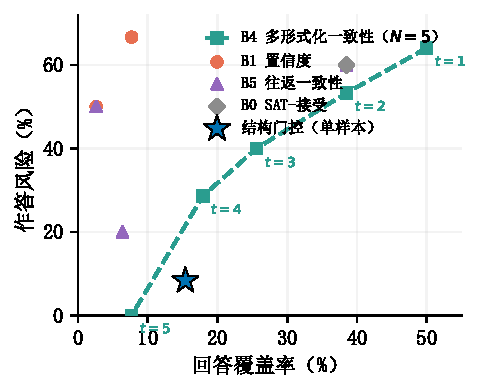
\includegraphics[width=0.95\columnwidth]{figures/fig_baseline_rc}
  \caption{结构门控与拒答基线的风险--覆盖率对比（同一批 GPT-4o-mini 无门控输出）。
  结构门控为单样本确定性单点；B4 多形式化一致性为 $N=5$ 温度采样、按 $t$-of-$N$ 扫描；
  B1／B5 为置信度／往返阈值扫描；B0 为不拒答。}
  \label{fig:baseline_rc}
\end{figure}

\begin{table}[ht]
  \centering
  \caption{代表性操作点（GPT-4o-mini，78 金标）。“样本”为所需形式化次数。}
  \label{tab:baseline-rc}
  \small
  \resizebox{\linewidth}{!}{%
  \begin{tabular}{lccc}
    \toprule
    信号 & 样本 & 覆盖率(\%) & 作答风险(\%) \\
    \midrule
    B0 SAT-接受              & 1 & 38.5 & 60.0 \\
    B1 置信度（$\tau{=}75$） & 1 & 2.6  & 50.0 \\
    B5 往返一致性（$\tau{=}25$） & 1 & 6.4 & 20.0 \\
    B4 多形式化一致性（$t{=}4$） & 5 & 17.9 & 28.6 \\
    B4 多形式化一致性（$t{=}5$） & 5 & 7.7  & 0.0 \\
    \textbf{B$\star$ 结构门控} & \textbf{1} & \textbf{15.4} & \textbf{8.3} \\
    \bottomrule
  \end{tabular}
  }
\end{table}

结构门控以\emph{单次}形式化取得 15.4\% 覆盖率、8.3\% 作答风险（图~\ref{fig:baseline_rc}、
表~\ref{tab:baseline-rc}）。B1 置信度在该弱形式化器上\emph{未见区分力}：各阈值作答风险
均为 50--67\%，与 SAT-接受相当；B5 往返一致性略优（$\tau{=}25$ 时 6.4\% 覆盖、20\%
风险），但覆盖率不足门控一半、风险仍为其两倍余，且需一次额外回译调用。B4 多形式化一致性需
$N=5$ 个样本，且只有在 $t=5$（全部一致）
才把风险压到 0\%、但覆盖率仅 7.7\%（门控的一半）；在与门控相近的覆盖率（$t=4$，17.9\%）
下 B4 风险为 28.6\%，约为门控的 3.4 倍。因此，在表~\ref{tab:baseline-rc} 报告的离散操作点中，
结构门控以单次形式化取得更低风险和相近或更高覆盖；这是一项样本内比较，不表示其在所有
阈值、模型或任务上都支配其他拒答规则（对照表~\ref{tab:baseline-props} 的代价--性质）。

说明：本对比样本量小，绝对计数为——门控 12 个作答中 1 错，B4（$t{=}4$）14 个作答中
4 错，B5（$\tau{=}25$）5 个作答中 1 错，B1（$\tau{=}75$）2 个作答中 1 错；各操作点之差
落在个位数计数的波动范围内，因此该对比是方向性的样本内证据，其统计确证需扩展到全部
200 金标题 $\times$ 3 次重复的冻结状态（留作后续工作）。B1 的“未见区分力”是该弱形式化器
上的观察，不排除更强模型或更好的置信度诱导下有效。在 GPT-4o、DeepSeek-V3.2 上重复本
对比（B1／B4／B5）留作后续工作；logprob 置信度（B2）受限于纯文本接口；直接答案自一致性
（B3）绕过形式化流水线、是与门控“零额外调用”卖点竞争最直接的免训练信号，其对比同样
列入后续工作。

\subsection{消融实验：候选补全预算}
\label{sec:budget-replay}

为观察候选补全的预算效应，我们对已完成的完整轨迹进行确定性前缀重放，将
补全预算从 $K=0$ 扫描至 $K=3$。重放固定已经发生的形式化、候选生成与冲突
处理，只改变第一次非唯一门控后的停止位置；它因此描述\emph{同一轨迹}上的
操作点，而不是冻结相同初始约束后的组件因果效应。

\begin{figure}[t]
  \centering
  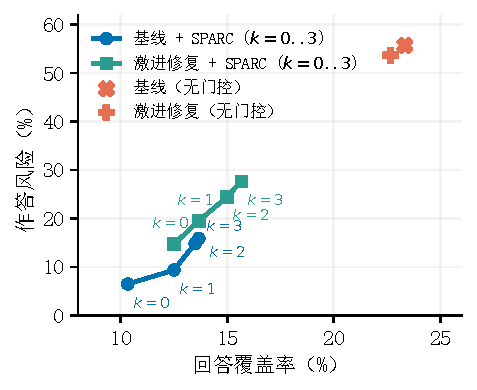
\includegraphics[width=0.95\columnwidth]{figures/fig_risk_coverage}
  \caption{补全预算 $K$ 的风险--覆盖率曲线。数据来自 200 个有标注问题的三次
  历史 API 重复的轨迹前缀重放。\method{} 曲线从 $K=0$ 的仅门控配置延伸至
  $K=3$ 的完整配置。}
  \label{fig:risk_coverage}
\end{figure}

在 baseline+\method{} 的已记录轨迹上，$K=0$ 时回答覆盖率为 10.33\%、
作答风险为 6.45\%；$K=3$ 时二者分别为 13.67\% 和 15.85\%。aggressive+
\method{} 的对应操作点从 12.50\%/14.67\% 变为 15.67\%/27.66\%。因此，
在这些已发生的轨迹中，补全预算增加了作答覆盖率，也接受了更多错误作答；
它并不构成补全会在相同初始约束上单调改善性能的证据。

\paragraph{受控配对补全消融。}为隔离补全的因果效应，我们冻结 baseline 无门控运行在
门控前的约束状态（200 个），在\emph{相同}初始约束上只改变补全预算。$K=0$（仅门控）
回答 20 题、作答风险 10.0\%（覆盖率 10.0\%）；$K=3$（门控＋补全）回答 28 题、风险
17.9\%（覆盖率 14.0\%）。补全把 8 个原本非唯一的状态转为作答，其中 5 个正确、3 个
错误。因此，在冻结相同初始约束的受控条件下，补全是覆盖率与风险之间的权衡而非单调
改善——它挽回部分作答，也接受了新的错误。该配对结果与轨迹重放方向一致，并在
单种子、200 个冻结状态的范围内支持这一权衡解释（脚本 \texttt{run\_frozen\_sparc.py}；
样本较小）。

答案变量集 $V_A$ 选择与求解超时策略的敏感性分析留作后续工作。

\subsection{其他实验与证据范围}

\paragraph{\sbw{} 随能力与难度的分布。}\label{sec:prevalence}SBW 并非均匀分布。在 GPT-4o-mini 上，作答的
SBW 率随网格规模从小格的 0--36\%（3$\times$3、3$\times$4）升到大格的 75--100\%
（4$\times$4、5$\times$3、6$\times$4）：形式化越难，线索遗漏与欠约束越多。跨形式化器
看，在\emph{相同}的困难网格（4$\times$4、5$\times$3、5$\times$4、6$\times$3、6$\times$4，
仅金标）上，SBW 率随能力下降但不消失——GPT-4o-mini 81\%、DeepSeek-V3.2 23\%、
GPT-4o 10\%（表~\ref{tab:sbw-capability}）；三者作答率相近（40--47\%），其余困难实例
形式化失败为显式非作答。更重要的是，强形式化器残余的 SBW 仍\emph{结构可检出}：
在当前困难网格样本中，GPT-4o-mini 的 \sbw{} 中 6/64 为唯一但错，因而逃逸唯一性门控；
两个更强形式化器的样本中未观察到此类逃逸。后者的 \sbw{} 计数较小，不能据此推断真实
逃逸率为零，也不足以比较不同模型上的门控收益。识别唯一但错的残余错误仍需要文本--
约束语义对齐。

\begin{table}[ht]
  \centering
  \caption{困难网格（4$\times$4、5$\times$3、5$\times$4、6$\times$3、6$\times$4，仅金标）上
  \sbw{} 随形式化器能力的分布。逃逸为唯一但错、门控无法检出的 \sbw{}。GPT-4o-mini 为
  三次重复合并，其余为单次运行；强形式化器的 \sbw{} 计数较小，方向性结论待更大样本确认。}
  \label{tab:sbw-capability}
  \small
  \resizebox{\linewidth}{!}{%
  \begin{tabular}{lcccc}
    \toprule
    形式化器 & 作答率(\%) & \sbw{} 率(\%) & 可检出 & 逃逸 \\
    \midrule
    GPT-4o-mini   & 40 & 81 & 58 & 6 \\
    DeepSeek-V3.2 & 47 & 23 & 7  & 0 \\
    GPT-4o        & 47 & 10 & 3  & 0 \\
    \bottomrule
  \end{tabular}
  }
\end{table}

\paragraph{跨任务诊断（AR-LSAT）。}为检验 \sbw{} 是否只出现在逻辑网格任务中，我们审计了
AR-LSAT~\cite{zhong2022} 的求解轨迹。1{,}630 条轨迹中，418 条可判定为答案错误、
122 条正确、900 条无法判定、190 条因信息不足跳过；在 540 条可判定 SAT 轨迹中，
错误占 77.4\%。这一观察仅支持“SAT 不是任务正确性的自动代理”这一诊断前提。
AR-LSAT 的结构谓词为选项良定模式，不同于 ZebraLogic 的唯一性，故本文不使用它
估计 \method{} 的方法效应，相关实现探针仅作附录审计。

\paragraph{探索性运行的证据范围。}\label{sec:exploratory-scope}%
本文的独立端到端臂、组件敏感性、基础模型与 AR-LSAT 运行都未冻结相同的
门控前状态或统一输出协议：例如 600 对有标注运行中，baseline 与 baseline+\method{}
只有 175 对（29.2\%）门控前约束多重集相同，aggressive 配置只有 199 对（33.2\%）
相同。这些运行可用于检查实现是否可运行，但不能支持修复收益、准确率提升或跨任务
泛化结论。为避免与主证据混淆，其完整账本（未配对端到端表、配对溯源审计、组件与
模型／任务敏感性、调用开销）作为审计材料单独归档，正文不据此作任何方法效应主张%
\ifincludeexploratory
（见附录~\ref{app:exploratory}）%
\fi
。


\section{局限性与讨论}
\label{sec:limitations}

\paragraph{结构条件不是语义验证。}
\method{} 只适用于任务规范能给出可信答案空间条件的场景。开放式生成、允许
多个等价方案的规划任务或先验本身不可靠的任务，不能直接套用唯一性门控。即使
先验有效，答案投影唯一但仍错误的 SAT 输出仍会通过检查：固定状态诊断中，
baseline 的 78 个 \sbw{} 有 6 个唯一，aggressive 的 73 个有 4 个唯一。识别
这些错误仍需要文本--约束语义对齐，而不能只依赖解空间形状。困难网格上的有限样本
显示，较强形式化器的 \sbw{} 率较低（\S\ref{sec:prevalence}）；但现有结果没有在相同
冻结状态上比较各模型的门控收益，因此不能据此排序该信号对不同模型或难度的实际价值。

\paragraph{接口和候选恢复的边界。}
本文报告的全部数字来自以全部非追踪整数变量近似 $V_A$ 的历史口径。当前实现已
机械支持从可见题面推导（不读 \texttt{puzzle.solution}）的答案变量白名单并默认
用于新运行（无匹配变量时回退到整数近似并记录口径）；白名单口径下对
表~\ref{tab:gate-diagnostic} 的离线重放属于免费的敏感性分析，留作后续工作。
其他任务若含整数辅助变量，必须显式指定答案投影。门控超时或无法构造
投影时，历史实现会兼容性放行，这类输出没有结构保证。候选的区分性验收只保证
排除至少一个当前完整模型，不保证答案投影收缩或候选忠实于原文；单元素冲突核
上的处理还可能替换新候选。因此，候选补全和冲突处理仍是启发式过程。

\paragraph{评测边界。}
固定状态结果应被理解为答案模式校验后的结构筛查，因为历史流水线从
\texttt{puzzle.solution} 读取了预期键名。ZebraLogic 也只有 200 个可评分实例，
三次历史 API 重复并非受控随机种子；题目聚类 bootstrap 不能解决未配对输入或
服务端版本漂移。AR-LSAT 的门控探针、GPT-4o 和组件探针未提供可比较的冻结状态，
因此不能支持跨模型或跨任务的方法泛化；AR-LSAT 仅以轨迹审计支持 SBW 的跨任务
诊断（\S\ref{sec:rq23}）。为此，本版本在 \S\ref{sec:setup} 增加去键名校验的门控
复算以量化对答案模式前置条件的依赖，并在 \S\ref{sec:baseline-cmp} 与口头置信度、往返
一致性和多形式化一致性等启发式拒答基线作风险--覆盖率对比~\cite{hall2026,singh2026}；跨模型、跨任务泛化
以及候选补全的冻结输入配对评估仍留待后续工作。

% ============================================================
\section{结论}
\label{sec:conclusion}

本文针对 LLM 约束形式化中的决策缺口——约束可满足并不足以接受其任务答案——提出
\method{}：它在答案变量上以一次带阻塞子句的增量求解检验答案投影是否唯一，把确定的
非唯一状态映射为结构性拒答，改变的是 SAT 后的接受接口而非语义验证器或修复器。在
ZebraLogic 冻结的无门控 SAT 状态上，唯一性探针在去键名保守口径下检出 baseline 与
aggressive 输出中 81.3\% 与 82.3\%（答案模式预校验口径下 92.3\% 与 94.5\%）的已观测
\sbw{}，代价是 9.7\% 与 23.8\% 的正确输出被拒答，少数唯一但错的输出仍会逃逸；在 78 个
金标题的小样本上，门控以单次形式化取得 15.4\% 覆盖率与 8.3\% 作答风险，可与口头置信度、
往返一致性和多形式化一致性基线在同一坐标系比较，而补全实验仅支持覆盖率与风险之间的
权衡。因此，现有证据支持将唯一答案任务的答案投影唯一性用作单样本、零额外
调用的 SAT 后拒答信号，但不支持语义正确性、端到端修复收益或跨任务泛化；后续工作应
机械执行答案变量白名单与 UNKNOWN 接口、对候选补全开展冻结输入的前瞻性配对评估，并
把该信号检验到其他唯一答案任务与基础模型。

% ============================================================
\begin{thebibliography}{99}

% ===== 神经符号推理（自旧稿复用，已核实）=====
\bibitem{pan2023}
Pan, L.; Albalak, A.; Wang, X.; and Wang, W.~Y. 2023.
Logic-LM: Empowering Large Language Models with Symbolic Solvers for Faithful Logical Reasoning.
In \textit{Findings of EMNLP 2023}, 3806--3824.

\bibitem{olausson2023}
Olausson, T.~X.; Gu, A.; Lipkin, B.; Zhang, C.; Solar-Lezama, A.; Tenenbaum, J.~B.; and Levy, R. 2023.
LINC: A Neurosymbolic Approach for Logical Reasoning by Combining Language Models with First-Order Logic Provers.
In \textit{Proc. EMNLP 2023}, 5153--5176.

\bibitem{ye2023}
Ye, X.; Chen, Q.; Dillig, I.; and Durrett, G. 2023.
SatLM: Satisfiability-Aided Language Models Using Declarative Prompting.
In \textit{Proc. NeurIPS 2023}, vol.~36.

% 2026-07-12 经 ACL Anthology 核实（作者拼写 Radhakrishna、NLRSE workshop 页码）
\bibitem{kirtania2024}
Kirtania, S.; Gupta, P.; and Radhakrishna, A. 2024.
LOGIC-LM++: Multi-Step Refinement for Symbolic Formulations.
In \textit{Proc. 2nd Workshop on Natural Language Reasoning and Structured
Explanations (NLRSE@ACL 2024)}, 56--63. arXiv:2407.02514.

\bibitem{kesseli2025}
Kesseli, P.; O'Hearn, P.; and Silveira Cabral, R. 2025.
Logic.py: Bridging the Gap between LLMs and Constraint Solvers.
arXiv:2502.15776.

\bibitem{callewaert2025}
Callewaert, B.; Vandevelde, S.; and Vennekens, J. 2025.
VERUS-LM: A Versatile Framework for Combining LLMs with Symbolic Reasoning.
In \textit{Proc. ICLP 2025}, EPTCS 439, 47--62.

\bibitem{singh2026}
Singh, V.; Cassel, D.; Weir, N.; Feng, N.; and Bayless, S. 2026.
VERGE: Formal Refinement and Guidance Engine for Verifiable LLM Reasoning.
arXiv:2601.20055.

% hall2026 / oh2026 于 2026-07-10 经 arXiv 页面核实（标题+作者+日期）
\bibitem{hall2026}
Hall, B.; and Eiers, W. 2026.
Neurosymbolic Auditing of Natural-Language Software Requirements.
arXiv:2605.13817.

\bibitem{oh2026}
Oh, H.; Stern, S.; Lee, Y.; and Philipose, M. 2026.
Neurosymbolic Language Reasoning as Satisfiability Modulo Theory.
arXiv:2602.18095.

% ===== NL→约束/优化建模（以下新增条目均于 2026-07-12 经
% arXiv / PMLR / Dagstuhl / ACL Anthology 页面核实标题、作者与 venue）=====
\bibitem{tsouros2023}
Tsouros, D.; Verhaeghe, H.; Kad{\i}o\u{g}lu, S.; and Guns, T. 2023.
Holy Grail 2.0: From Natural Language to Constraint Models.
arXiv:2308.01589.

\bibitem{michailidis2024}
Michailidis, K.; Tsouros, D.; and Guns, T. 2024.
Constraint Modelling with LLMs Using In-Context Learning.
In \textit{Proc. CP 2024}, LIPIcs vol.~307, 20:1--20:27.

\bibitem{ahmaditeshnizi2024}
AhmadiTeshnizi, A.; Gao, W.; and Udell, M. 2024.
OptiMUS: Scalable Optimization Modeling with (MI)LP Solvers and Large
Language Models. In \textit{Proc. ICML 2024}, PMLR 235, 577--596.

\bibitem{wei2025}
Wei, A.; Wu, Y.; Wan, Y.; Suresh, T.; Tan, H.; Zhou, Z.; Koyejo, S.;
Wang, K.; and Aiken, A. 2025.
SATBench: Benchmarking LLMs' Logical Reasoning via Automated Puzzle
Generation from SAT Formulas. In \textit{Proc. EMNLP 2025}, 33832--33849.

% ===== LLM 自修复（huang2024/olausson2024 于 2026-07-10 经 web 核实）=====
\bibitem{madaan2023}
Madaan, A.; Tandon, N.; Gupta, P.; et al. 2023.
Self-Refine: Iterative Refinement with Self-Feedback.
In \textit{Proc. NeurIPS 2023}, vol.~36.

\bibitem{shinn2023}
Shinn, N.; Cassano, F.; Labash, B.; Gopinath, A.; and Narasimhan, K. 2023.
Reflexion: Language Agents with Verbal Reinforcement Learning.
In \textit{Proc. NeurIPS 2023}, vol.~36.

\bibitem{huang2024}
Huang, J.; Chen, X.; Mishra, S.; Zheng, H.~S.; Yu, A.~W.; Song, X.; and Zhou, D. 2024.
Large Language Models Cannot Self-Correct Reasoning Yet.
In \textit{Proc. ICLR 2024}. arXiv:2310.01798.

\bibitem{olausson2024}
Olausson, T.~X.; Inala, J.~P.; Wang, C.; Gao, J.; and Solar-Lezama, A. 2024.
Is Self-Repair a Silver Bullet for Code Generation?
In \textit{Proc. ICLR 2024}. arXiv:2306.09896.

% ===== 优化建模的求解器诊断与语义修复（2026-07-12 经 arXiv 核实）=====
\bibitem{chen2024optichat}
Chen, H.; Constante-Flores, G.~E.; and Li, C. 2024.
Diagnosing Infeasible Optimization Problems Using Large Language Models.
\textit{INFOR: Information Systems and Operational Research} 62(4).
arXiv:2308.12923.

% arXiv 页标注 ICML 2026 接收；投稿前按正式 proceedings 复核 venue
\bibitem{zhang2025sacopt}
Zhang, Y.; Kang, Q.; Chen, Y.; Wang, Y.; Han, X.; Zhong, T.; Yuan, M.;
and Ma, C. 2025.
SAC-Opt: Semantic Anchors for Iterative Correction in Optimization
Modeling. arXiv:2510.05115.

\bibitem{ao2026}
Ao, R.; Simchi-Levi, D.; and Wang, X. 2026.
OptiRepair: Closed-Loop Diagnosis and Repair of Supply Chain Optimization
Models with LLM Agents. arXiv:2602.19439.

% ===== 自动形式化忠实性验证（2026-07-12 经 arXiv/OpenReview 核实）=====
\bibitem{wu2022}
Wu, Y.; Jiang, A.~Q.; Li, W.; Rabe, M.~N.; Staats, C.; Jamnik, M.; and
Szegedy, C. 2022.
Autoformalization with Large Language Models.
In \textit{Proc. NeurIPS 2022}, vol.~35.

\bibitem{lu2025}
Lu, J.; Wan, Y.; Huang, Y.; Xiong, J.; Liu, Z.; and Guo, Z. 2025.
FormalAlign: Automated Alignment Evaluation for Autoformalization.
In \textit{Proc. ICLR 2025}. arXiv:2410.10135.

\bibitem{li2024symbolic}
Li, Z.; Wu, Y.; Li, Z.; Wei, X.; Zhang, X.; Yang, F.; and Ma, X. 2024.
Autoformalize Mathematical Statements by Symbolic Equivalence and
Semantic Consistency. In \textit{Proc. NeurIPS 2024}. arXiv:2410.20936.

\bibitem{ryu2025}
Ryu, H.; Kim, G.; Lee, H.~S.; and Yang, E. 2025.
Divide and Translate: Compositional First-Order Logic Translation and
Verification for Complex Logical Reasoning.
In \textit{Proc. ICLR 2025}. arXiv:2410.08047.

\bibitem{raza2025}
Raza, M.; and Milic-Frayling, N. 2025.
Instantiation-based Formalization of Logical Reasoning Tasks using
Language Models and Logical Solvers.
In \textit{Proc. IJCAI 2025}. arXiv:2501.16961.

\bibitem{zhou2024dtv}
Zhou, J.~P.; Staats, C.; Li, W.; Szegedy, C.; Weinberger, K.~Q.; and
Wu, Y. 2024.
Don't Trust: Verify --- Grounding LLM Quantitative Reasoning with
Autoformalization. In \textit{Proc. ICLR 2024}. arXiv:2403.18120.

% ===== 程序合成 / 约束获取（bessiere2013 于 2026-07-10 经 web 核实）=====
% 2026-07-12 jha2010 按标准条目补全页码；投稿前 DBLP 复核。
\bibitem{jha2010}
Jha, S.; Gulwani, S.; Seshia, S.~A.; and Tiwari, A. 2010.
Oracle-Guided Component-Based Program Synthesis.
In \textit{Proc. ICSE 2010}, 215--224.

\bibitem{bessiere2013}
Bessiere, C.; Coletta, R.; Hebrard, E.; Katsirelos, G.; Lazaar, N.; Narodytska, N.; Quimper, C.-G.; and Walsh, T. 2013.
Constraint Acquisition via Partial Queries.
In \textit{Proc. IJCAI 2013}.

% 2026-07-12 经 AAAI OJS 页面核实
\bibitem{tsouros2024}
Tsouros, D.; Berden, S.; and Guns, T. 2024.
Learning to Learn in Interactive Constraint Acquisition.
In \textit{Proc. AAAI 2024}, 8154--8162.

% ===== 解空间技术 / 评测端唯一性 =====
\bibitem{liffiton2008}
Liffiton, M.~H.; and Sakallah, K.~A. 2008. Algorithms for Computing Minimal
Unsatisfiable Subsets of Constraints. \textit{J. Automated Reasoning} 40(1):1--33.

\bibitem{amonkar2025}
Amonkar, R.; Kayan, C.~E.; Lai, Q.; Le Bras, R.; and Zhang, L. 2025.
A Reality Check of Language Models as Formalizers on Constraint Satisfaction Problems.
arXiv:2505.13252.

% ===== Selective prediction =====
% 2026-07-12 按标准条目补全卷期页码；投稿前 DBLP 复核。
\bibitem{chow1957}
Chow, C.~K. 1957.
An Optimum Character Recognition System Using Decision Functions.
\textit{IRE Trans. Electronic Computers} EC-6(4): 247--254.

% ===== 选择性预测 / LLM 拒答 / 一致性信号（以下条目于 2026-07-12
% 经 arXiv / ACL Anthology / NeurIPS proceedings 核实）=====
\bibitem{geifman2017}
Geifman, Y.; and El-Yaniv, R. 2017.
Selective Classification for Deep Neural Networks.
In \textit{Proc. NeurIPS 2017}, vol.~30.

\bibitem{kamath2020}
Kamath, A.; Jia, R.; and Liang, P. 2020.
Selective Question Answering under Domain Shift.
In \textit{Proc. ACL 2020}, 5684--5696.

\bibitem{zhang2024rtuning}
Zhang, H.; Diao, S.; Lin, Y.; Fung, Y.~R.; Lian, Q.; Wang, X.; Chen, Y.;
Ji, H.; and Zhang, T. 2024.
R-Tuning: Instructing Large Language Models to Say `I Don't Know'.
In \textit{Proc. NAACL 2024}. arXiv:2311.09677.

\bibitem{xiong2024}
Xiong, M.; Hu, Z.; Lu, X.; Li, Y.; Fu, J.; He, J.; and Hooi, B. 2024.
Can LLMs Express Their Uncertainty? An Empirical Evaluation of Confidence
Elicitation in LLMs. In \textit{Proc. ICLR 2024}. arXiv:2306.13063.

% TACL 正式卷期页码投稿前从 MIT Press 页面补齐
\bibitem{wen2024}
Wen, B.; Yao, J.; Feng, S.; Xu, C.; Tsvetkov, Y.; Howe, B.; and
Wang, L.~L. 2024.
Know Your Limits: A Survey of Abstention in Large Language Models.
\textit{Trans. ACL}. arXiv:2407.18418.

\bibitem{wang2023}
Wang, X.; Wei, J.; Schuurmans, D.; Le, Q.; Chi, E.; Narang, S.;
Chowdhery, A.; and Zhou, D. 2023.
Self-Consistency Improves Chain of Thought Reasoning in Language Models.
In \textit{Proc. ICLR 2023}.

\bibitem{manakul2023}
Manakul, P.; Liusie, A.; and Gales, M.~J.~F. 2023.
SelfCheckGPT: Zero-Resource Black-Box Hallucination Detection for
Generative Large Language Models. In \textit{Proc. EMNLP 2023}.

% ===== 基准 =====
\bibitem{lin2025}
Lin, B.~Y.; Xie, J.; Tiwari, A.; and Durrett, G. 2025.
ZebraLogic: Benchmarking Logical Reasoning in Large Language Models.
In \textit{Proc. ICML 2025}.

\bibitem{zhong2022}
Zhong, W.; Cui, R.; Guo, Y.; Qi, Y.; Zhang, Y.; Liu, Z.; Wang, S.; Chen, J.; Duan, N.; Yang, M.; and Yao, Y. 2022.
AR-LSAT: Investigating Analytical Reasoning of Text.
In \textit{Findings of NAACL 2022}, 1672--1686.

\bibitem{tyagi2024}
Tyagi, N.; Parmar, M.; Kulkarni, M.; et al. 2024.
Step-by-Step Reasoning to Solve Grid Puzzles: Where do LLMs Falter?
In \textit{Proc. EMNLP 2024}, 19863--19878.

% ===== SMT =====
\bibitem{demoura2008}
de Moura, L.; and Bj\o{}rner, N. 2008. Z3: An Efficient SMT Solver.
In \textit{Proc. TACAS}, LNCS vol.~4963, 337--340. Springer.

\end{thebibliography}

% ============================================================
\appendix

\section{实现细节}
\label{app:impl}

求解器使用 \zthree~\cite{demoura2008} Python API。约束通过
\texttt{assert\_and\_track} 加入求解器，追踪变量用于提取 UNSAT core。
本文报告的运行以模型中的全部非追踪整数变量构造唯一性阻塞子句；这是一个
基准特定的投影近似。当前实现默认改用从可见题面推导的答案变量白名单
（\texttt{--sparc-va-mode}，无匹配时回退到整数近似并在 trace 中记录口径），
但该口径未用于本文任何报告数字。差分摘要最多展示 12 个答案
变量上取值不同的变量；每轮补全最多生成两个候选。候选必须通过语法解析并
区分当前两个完整模型，但实现不限制候选只能引用答案变量。主实验设置
$K=3$、$R=2$。

\paragraph{候选优先的冲突处理。}候选补全可能与早期误译冲突。若直接以恢复
SAT 为目标，处理程序可能删除或弱化刚加入的候选，从而撤销触发冲突的线索。
为避免这一路径，当 UNSAT core 中存在其他约束时，\method{} 优先将这些早期约束
交给 LLM 修改，并提示其不要删除或弱化新候选，每次处理后重新求解，最多执行 $R$
轮。这是一项候选优先的启发式策略，而非机械不变量：若新候选是 core 的唯一成员，
实现会回退为将整个 core 交给处理例程以避免停滞，该例程仍可能替换新候选。因此
本文不声称候选永远受保护，也不将此模块作为端到端修复效果的证据；任何处理后的
SAT 状态都必须再次经过结构门控，UNKNOWN 仍按兼容输出策略单独记录。

门控检测到多解且预算耗尽时，最终状态记为
\path{SAT_NONUNIQUE}。UNSAT、\path{INVALID_MODEL}、
\path{KEY_MISMATCH} 和翻译失败保留各自状态。评测只对官方答案非空的
200 个问题计算正确率。答案比较将键转为小写并移除非字母数字字符，同时
规范化房间编号；预测必须覆盖全部真值键并逐项相等。唯一性求解返回
UNKNOWN 时，历史实现会保留基础流水线答案并记录标记；该状态不计为确定的
结构门控通过。

\section{候选补全的形式化细节}
\label{app:completion}

实现把差异集合 $D$ 的两组取值、原题与当前约束一并提供给 LLM，要求返回一条候选
约束 $c^{*}$，并机械验收其至少排除两个当前模型之一：
\begin{equation}
  \lnot\bigl(M\models c^{*}\ \wedge\ M'\models c^{*}\bigr).
  \label{eq:discriminate}
\end{equation}
未能区分两个模型的候选被拒绝，至多重试一次。我们对该分支只作一个有限进展的陈述。

\begin{proposition}[区分性候选的完整模型空间收缩]
\label{prop:full-model-contraction}
设 $M,M'\in\Sol(C)$，候选 $c^{*}$ 满足式~\eqref{eq:discriminate}，且
$C\cup\{c^{*}\}$ 为 SAT，则
$\Sol(C\cup\{c^{*}\})\subsetneq\Sol(C)$。
\end{proposition}
\begin{proof}
加入 $c^{*}$ 只会从 $\Sol(C)$ 中筛除模型，故包含关系成立。式~\eqref{eq:discriminate}
保证 $M$ 或 $M'$ 至少有一个不满足 $c^{*}$，因此至少一个原有模型被移除；SAT 条件
保证补全后的模型空间非空，故该包含关系为严格包含。
\end{proof}

有限预算 $K$ 保证该探索过程终止。该命题只陈述完整模型空间的严格收缩，不意味着
答案投影收缩、候选忠实于原文或最终答案正确。

\section{逐重复结果}
\label{app:accounting}

表~\ref{tab:per-seed} 给出主表的逐重复分解。42、123 和 7 是历史目录
标识，并非已传入服务端的随机种子。其他非作答不包含
\texttt{SAT\_NONUNIQUE}，因此每行四类结果之和为 200。

\begin{table}[t]
  \centering
  \caption{ZebraLogic 逐次独立 API 重复的完整结果账本。base=baseline，agg=aggressive，S=SPARC。}
  \label{tab:per-seed}
  \small
  \renewcommand{\arraystretch}{0.84}
  \setlength{\tabcolsep}{3pt}
  \begin{tabular}{clrrrrr}
    \toprule
    ID & 系统 & 正确 & \sbw{} & 拒答 & 其他 & Acc \\
    \midrule
    42  & base  & 21 & 25 & 0  & 154 & 10.5 \\
        & base+S & 23 & 5  & 16 & 156 & 11.5 \\
        & agg   & 20 & 25 & 0  & 155 & 10.0 \\
        & agg+S  & 26 & 7  & 13 & 154 & 13.0 \\
    \midrule
    123 & base  & 19 & 28 & 0  & 153 & 9.5 \\
        & base+S & 23 & 4  & 18 & 155 & 11.5 \\
        & agg   & 21 & 26 & 0  & 153 & 10.5 \\
        & agg+S  & 21 & 8  & 17 & 154 & 10.5 \\
    \midrule
    7   & base  & 22 & 25 & 0  & 153 & 11.0 \\
        & base+S & 23 & 4  & 17 & 156 & 11.5 \\
        & agg   & 22 & 22 & 0  & 156 & 11.0 \\
        & agg+S  & 21 & 11 & 13 & 155 & 10.5 \\
    \bottomrule
  \end{tabular}
\end{table}

\enlargethispage{3\baselineskip}

% ============================================================
\ifincludeexploratory
\section{探索性审计账本}
\label{app:exploratory}

\subsection{\sbw{} 发生率与未配对端到端账本（描述性）}
\label{sec:main}

\begin{table}[ht]
  \centering
  \caption{ZebraLogic 的端到端结果账本。计数来自 200 个有标注问题的三次
  独立 API 重复，共 600 次运行。Acc、Cov 和 Risk 分别表示总体准确率、回答覆盖率和
  作答风险。各臂独立生成门控前形式化，因而本表描述系统臂分布，而非配对方法效应。
  每行四类结果计数之和为 600。}
  \label{tab:main}
  \small
  \resizebox{\linewidth}{!}{%
  \begin{tabular}{lrrrrrrr}
    \toprule
    系统 & Acc(\%) & 正确 & \sbw{} & 结构性拒答 & 其他非作答 & Cov(\%) & Risk(\%) \\
    \midrule
    baseline                    & 10.33 & 62 & 78 & 0  & 460 & 23.33 & 55.71 \\
    baseline+\method            & 11.50 & 69 & 13 & 51 & 467 & 13.67 & 15.85 \\
    aggressive                  & 10.50 & 63 & 73 & 0  & 464 & 22.67 & 53.68 \\
    aggressive+\method          & 11.33 & 68 & 26 & 43 & 463 & 15.67 & 27.66 \\
    \bottomrule
  \end{tabular}}
\end{table}

RQ1 显示，两个无门控系统都产生了大量 \sbw{}。baseline 在 600 次运行中
回答 140 次，其中 78 次来自 SAT 状态的错误作答；aggressive 回答 136 次，
其中 73 次错误。相应作答风险为 55.71\% 和 53.68\%。三次历史 API 重复的
\sbw{} 计数分别为 25、28、25（baseline）和 25、26、22（aggressive）。
因此，在这一运行条件下，SAT 输出不能作为任务答案正确的充分代理。

表~\ref{tab:main} 还记录了含 \method{} 的独立端到端臂。baseline+\method{}
的 \sbw{} 计数为 13，aggressive+\method{} 为 26，相应作答风险为 15.85\%
和 27.66\%。这些数同时伴随覆盖率收缩：对应的回答覆盖率为 13.67\% 和
15.67\%，而无门控臂为 23.33\% 和 22.67\%。其中“结构性拒答”只统计
\texttt{SAT\_NONUNIQUE}；UNSAT、解析失败等其他非作答保持单独计数，
不会被误记为主动拒答。该账本的可解释性取决于下一节的溯源审计。

以题目聚类的 95\% bootstrap 区间计，四个臂的风险依次为 55.7\%
[42.6\%, 68.6\%]、15.9\% [5.8\%, 28.4\%]、53.7\%
[40.4\%, 66.7\%] 和 27.7\% [15.6\%, 41.0\%]；覆盖率区间依次为
[17.8\%, 29.2\%]、[9.3\%, 18.2\%]、[17.0\%, 28.5\%] 与
[11.0\%, 20.8\%]。总体准确率点估计分别为 10.33\%、11.50\%、
10.50\% 和 11.33\%，相应区间重叠。这些区间只描述各臂的观测分布，
不能据此归因于门控或补全，也不支持准确率提升主张。

\subsection{配对与溯源审计}
\label{sec:pairing-audit}

为检验端到端臂是否共享相同输入，我们从 trace 重建每次运行在第一次门控前
的实际约束状态：显式快照覆盖旧状态，已接受修复执行约束替换；比较时忽略
约束顺序但保留重复约束。表~\ref{tab:pairing-audit} 显示，600 对有标注运行中，
baseline 与 baseline+\method{} 只有 175 对（29.2\%）约束多重集相同，
aggressive 配置只有 199 对（33.2\%）相同。因此，表~\ref{tab:main} 的系统臂
虽配置对应，却不是门控前输入配对实验。

\begin{table}[ht]
  \centering
  \caption{端到端臂的门控前约束配对审计。\sbw{} 计数只针对事后筛得的
  相同约束子集，不代表预先设计的配对效应。}
  \label{tab:pairing-audit}
  \small
  \begin{tabular}{lrrrr}
    \toprule
    比较 & 全部对数 & 相同约束 & 比例(\%) & 子集 \sbw{}（前/后） \\
    \midrule
    baseline / baseline+\method{}     & 600 & 175 & 29.2 & 21 / 6 \\
    aggressive / aggressive+\method{} & 600 & 199 & 33.2 & 19 / 8 \\
    \bottomrule
  \end{tabular}
\end{table}

在相同约束子集中，\sbw{} 仍呈较低计数，这与结构门控的预期方向一致；但该
子集是在观察两个臂后按约束相同筛选，可能改变样本构成，不能替代前瞻性冻结
输入实验。后续组件因果评估必须先缓存门控前约束，再在同一状态上运行各变体。

\subsection{基于完整轨迹的预算重放（条件性）}

图~\ref{fig:risk_coverage} 使用完整轨迹的确定性前缀重放，将补全预算从
$K=0$ 扫描到 $K=3$。这项分析固定每条完整轨迹已经发生的形式化、候选生成和
修复结果，只改变第一次非唯一门控后的停止预算。增加预算既能挽回部分作答，
也会接受更多错误作答；因此 $K$ 选择风险与覆盖率之间的操作点，而不是单调
改善所有指标。

（风险--覆盖率曲线见正文图~\ref{fig:risk_coverage}。）

\paragraph{补全预算。}
\label{sec:ablation}

若某次运行在第 $c$ 次补全后得到确定的结构门控通过，则 $K\geq c$ 时保留
原答案，$K<c$ 时在对应门控位置返回非作答。$K=3$ 的重放逐项复现
表~\ref{tab:main} 中的 \method{} 账本。这说明重放没有外推未发生的轨迹，
但它不能隔离“若从同一初始约束重新运行，补全会造成什么变化”。

\begin{table}[ht]
  \centering
  \caption{补全预算的完整轨迹前缀重放。每个系统包含 600 次运行；非作答包含
  结构性拒答和其他失败状态。该分析改变停止预算，不是冻结输入的组件消融。}
  \label{tab:ablation}
  \small
  \begin{tabular}{lrrrrrr}
    \toprule
    系统 & $K$ & 正确 & \sbw{} & 非作答 & Cov(\%) & Risk(\%) \\
    \midrule
    baseline+\method   & 0 & 58 & 4  & 538 & 10.33 & 6.45 \\
                         & 1 & 68 & 7  & 525 & 12.50 & 9.33 \\
                         & 2 & 69 & 12 & 519 & 13.50 & 14.81 \\
                         & 3 & 69 & 13 & 518 & 13.67 & 15.85 \\
    \midrule
    aggressive+\method & 0 & 64 & 11 & 525 & 12.50 & 14.67 \\
                         & 1 & 66 & 16 & 518 & 13.67 & 19.51 \\
                         & 2 & 68 & 22 & 510 & 15.00 & 24.44 \\
                         & 3 & 68 & 26 & 506 & 15.67 & 27.66 \\
    \bottomrule
  \end{tabular}
\end{table}

在 baseline+\method{} 轨迹上，$K=0$ 的风险为 6.45\%，但只回答 10.33\%
的运行。将 $K$ 从 0 增至 3 后，正确回答由 58 增至 69，\sbw{} 由 4 增至
13；aggressive 轨迹呈现同方向变化。因而，这些已发生轨迹上的补全预算主要
改变覆盖率与风险之间的权衡，不能被解释为所有初始状态上的单调改进。

\subsection{组件敏感性运行（探索性）}

预算重放只隔离同一完整轨迹上的停止预算。为观察差分提示与候选优先策略在另一组
运行中的行为，我们在 legacy-42 配置上独立运行两个变体：
\textbf{盲补全}（补全提示不含模型差分摘要，且不执行区分性验收）与
\textbf{无候选优先处理}（冲突处理不优先新补全约束、去除禁止弱化指令）。
表~\ref{tab:component} 给出 200 个有标注题上的结果账本。这里“匹配”只指
超参数相同：完整系统与盲补全只有 66/200 个运行共享相同门控前约束，与
无保护修复只有 62/200 个共享相同约束。因此，该表不能隔离单个开关的因果效应。

\begin{table}[ht]
  \centering
  \caption{组件敏感性运行（legacy-42，有标注 $n=200$）。各臂配置相同但
  形式化独立生成，不构成冻结输入的因果消融。}
  \label{tab:component}
  \small
  \begin{tabular}{lrrrrrr}
    \toprule
    系统 & 正确 & \sbw{} & 结构性拒答 & 其他非作答 & Cov(\%) & Risk(\%) \\
    \midrule
    完整 \method   & 23 & 5 & 16 & 156 & 14.00 & 17.86 \\
    盲补全         & 21 & 3 & 19 & 157 & 12.00 & 12.50 \\
    无保护修复     & 23 & 2 & 18 & 157 & 12.50 & 8.00 \\
    \bottomrule
  \end{tabular}
\end{table}

机制层统计使用的是全部 640 题 trace，因而分母不同于表~\ref{tab:component}
的 200 个有标注题。盲补全取消区分性验收后，665 个补全候选全部被接受；
完整系统则接受 234 个、拒绝 379 个。相应地，盲补全记录到 197 次冲突修复、
979 次门控求解和 132 次唯一性收敛，完整系统分别为 62、590 和 151 次；
每题 LLM 调用为 3.55 对 3.20。这个模式与“差分摘要和区分性验收会改变
搜索轨迹”的预期一致，但由于多数上游约束不同，不能把差异解释为组件效应，
更不能据此验证语义修复。

无保护修复与完整系统的机制记录接近：冲突修复为 67 对 62 次，接受补全为
227 对 234 个；200 题账本的正确回答同为 23，\sbw{} 为 2 对 5。在当前
基准、预算和样本规模下，保护路径的独立效应不可检出。因此，本文仅把该规则
视为降低候选被立即撤销倾向的启发式设计，而非保护不变量。差分提示与候选
优先策略仍需在冻结相同门控前约束后进行前瞻性配对重跑。

\subsection{模型与任务敏感性（探索性）}
\label{sec:gpt4o}

\begin{table}[ht]
  \centering
  \caption{不同基础模型在 baseline 配置下的单次结果（legacy-42 标识，同一批 200 个
  有标注问题）。}
  \label{tab:gpt4o}
  \small
  \begin{tabular}{lrrrrr}
    \toprule
    模型 & Acc(\%) & 正确 & \sbw{} & Cov(\%) & Risk(\%) \\
    \midrule
    GPT-4o-mini & 10.5 & 21 & 25 & 23.0 & 54.35 \\
    GPT-4o      & 25.5 & 51 & 4  & 27.5 & 7.27 \\
    \bottomrule
  \end{tabular}
\end{table}

在该单次 baseline 运行中，GPT-4o 的 \sbw{} 数量为 4，GPT-4o-mini 为 25。
这说明 \sbw{} 的观测频率会随基础形式化器和运行条件变化，但两个模型、各一次
运行不足以建立能力规律。现有 GPT-4o 的 \method{} 运行使用 aggressive 配置，
与表~\ref{tab:gpt4o} 的 baseline 不匹配，因此不用于估计方法效应。

AR-LSAT 的轨迹审计（1{,}630 条轨迹、540 条可判定 SAT 中 77.4\% 错误）已提至正文
\S\ref{sec:rq23} 作为 SBW 的跨任务诊断证据；此处仅补充其门控实现探针。我们在
AR-LSAT 测试集前 40 题运行了良定门控的实现探针。门控系统回答
16 题，其中 15 题正确、1 题错误；有 1 个正确答案在一次背景补全后恢复。
基线的 22/40 个正确结果包含 14 个随机回退答案，其中仅 2 个正确；若仅计算
求解器导出的 26 个答案，则为 20 个正确、6 个错误。两臂只有 11/40 个重建
背景约束多重集相同，且输出协议不同。因此这些数只说明该任务上的实现可运行，
不能比较风险、归因于门控，或支持跨数据集有效性结论。

\subsection{调用开销}
\label{sec:efficiency}

在完整 640 题历史 trace 中，baseline+\method{} 的三次配置平均每题记录
0.91 至 0.94 次结构门控探测，以及 0.36 至 0.39 次已接受补全后的重求解；
aggressive+\method{} 的对应范围为 0.78 至 0.80 和 0.31 至 0.35。与其
无门控配置相比，记录的 LLM 请求数高 0.86 至 1.07 次每题，但由于两臂的
上游形式化未配对，这些只是配置级描述，不能解释为 \method{} 的因果开销。
trace 显式记录 3{,}344 条候选处理事件，其中 1{,}336 条被接受、2{,}008 条
因未能区分当前模型而被显式拒绝。解析失败会被静默跳过，未包含在该拒绝计数
中；候选优先冲突处理共触发 347 次。

运行日志时间戳给出的墙钟范围为：baseline 20.1 至 22.7 秒每题，
baseline+\allowbreak\method{} 为 24.1 至 26.8 秒；aggressive 为 20.1 至
22.7 秒，aggressive+\allowbreak\method{} 为 24.0 至 26.5 秒。这些值包含
共享 API 的排队时间，且来自未配对的历史配置，不应被报告为可归因的时延增量。
调用计数与时长的汇总脚本见附录复现信息。

\fi
\end{document}
